%\documentclass[12pt]{amsart}
\documentclass[prbg,preprint]{revtex4-1} 
%Manuscripts that demonstrate new relations between apparently unrelated areas of physics are appropriate.
\usepackage{geometry} % see geometry.pdf on how to lay out the page. There's lots.
\usepackage{graphicx}
\usepackage{subcaption}
\usepackage{bm}
%\usepackage{subfig}
\usepackage{mathtools}
\usepackage{svg}
\geometry{a4paper} % or letter or a5paper or ... etc
\newcommand{\cvec}[1]{\rm{\bf{#1}}}
% \geometry{landscape} % rotated page geometry

% See the ``Article customise'' template for come common customisations

%\date{} % delete this line to display the current date

%%% BEGIN DOCUMENT
\begin{document}

\title{Dynamics of Two Freely Rotating Dipoles}
\author{Peter T. Haugen}
\author{Boyd F. Edwards}
%\affil[1]{Utah State University}
%\setcounter{Maxaffil}{0}
\maketitle
%\tableofcontents

\section{Abstract}
	The equations of motion for two spherical dipoles moving freely in a plane are arrived at. Special consideration is given to the contact state. Their equilibria are determined, small amplitude motion examined and large amplitude motion investigated to reveal that possible motions are exclusively quasi-periodic.
	Two distinct modes are identified one of which is isomorphic with the simple pendulum complete with continual spinning at high enough energy.
%	A subset of the motions are isomorphic with the simple pendulum including the transition to freely rotating with arbitrary amounts of kinetic energy.
	
\section{Introduction}
A system composed of two unrestricted spherical magnetic dipoles presents an interesting and fundamental set of phenomenon as two magnetic dipoles is amongst the simplest non-trivial macroscopic magnetic systems. Understanding their dynamics could prove useful in contexts such as the large dipole field proposed to provide a solar wind umbrella for Mars\cite{2017LPICo1989.8250G} or small magnetic toothless-gears\cite{doi:10.1119/1.5029823}.
While a numerically integrable method exists for calculating torques for radially oriented multi-pole cylinders\cite{Furlani:1995aa}  analytic techniques provide a useful check.

\begin{figure}[h]
  \centering
  \includegraphics[width=.85\linewidth]{./images/coordinates_scalable_2.pdf}
%overlapping hatching just doesn't render, swapped for banded solids  
  \caption{Schematic of labeling system describing two spheres in the plane featuring both the independent coordinates and the center of mass coordinates.}
\end{figure}


\section{Describing the System}
Intrinsic properties of the two dipoles are: their respective radii, which we shall label as $a_1$ and $a_2$, their masses, $m_1$ and $m_2$, and magnitudes of their dipole moments, $\mu_1$ and $\mu_2$.
\subsection{Coordinates}
\subsubsection{Cartesian}

Each of the dipoles has a location constrained to the x-y plane $\cvec{r_1}$ and $\cvec r_2$ along with an orientation for the dipole $\phi_1$ and $\phi_2$ which we will also constrain to the x-y plane, measured from the x-axis.
\subsubsection{Center Of Mass}
We can define a set of composite coordinates and quantities more appropriate for analyzing two-body system using the aforementioned independent coordinates a la Taylor's mechanics \cite{taylor2005classical}. 

The total and reduced mass

\begin{equation}
m_t = m_1+m_2
\qquad
m_r = \frac{m_1m_2}{m_1+m_2}
\end{equation}

The center of mass 
\begin{equation}
\cvec R = \frac{m_1 \cvec r_1+m_2 \cvec r_2}{m_t}
\end{equation}

And the displacement of dipole 2 from dipole 1
\begin{equation}
\cvec{r}
=  \cvec r_2-\cvec r_1 
= \textrm{r} [\cos(\theta) \hat {\cvec x}+\sin(\theta) \hat {\cvec y}]
\end{equation}


\subsection{Hamiltonian}
To take advantage of the numerous analytic techniques that can be applied to a system's Hamiltonian, it must first be calculated. Which in turn requires that we find its kinetic and potential energy in terms of its coordinates.
%BFE:We use the hamiltonian approach to find the equations of motion.
%PTH: Does this get at why? If the paper is supposed to have pedagogical value being a bit wordier to convey motive for rationale is important. 
\subsubsection{Energies}
The kinetic energy, T, in the center of mass coordinates can be found to be
%citing taylor mechanics for the reduced kinetic
\begin{equation}
T = \frac{1}{2}(
	m_t \dot R^2
	+m_r \dot r^2
	+m_r r^2 \dot \theta^2
	+ I_1 \dot \phi_1^2
	+ I_2 \dot \phi_2^2
)
\end{equation}
%BFE:rederive kinetic energy 
%PTH: or cite taylor's result have done the derivation before but this paper is already a bit long of tooth and we want to get to the novelty sooner rather than later
The potential energy for dipole 1 is merely its dot product with the local field, which in this case is caused entirely by dipole 2.
\begin{equation}
U_1 = -\boldsymbol \mu_1 \cdot \cvec B_2
\end{equation}

With the magnetic field for a dipole at some point of interest $\cvec r_i$ being given by \cite{griffiths2013introduction}
%PTH: isn't it a complete sentence if equation 6 is understood to be a noun? The alternative would just be having lots of sentences ending with "the following equation." leading to repetitive text. Possible middle ground, give all equations reference numbers and use that as the noun explicitly, now it isn't redundant and it will be formatting agnostic.

\begin{equation}
\cvec B_2 = 
\frac{\mu_0}{4\pi}\left[
	3\frac{\boldsymbol \mu_2 \cdot (\cvec r_i - \cvec r_2)}{|\cvec r_i - \cvec r_2|^5}(
	\cvec r_i - \cvec r_2
	)
	-\frac{\boldsymbol \mu_2}{|\cvec r_i - \cvec r_2|^3}
\right]
\end{equation}

Using our definition for $\cvec r$ we can simplify the potential down to

\begin{equation}
U_1 = 
\frac{\mu_0}{4\pi}
\frac{1}{r^3}\left[
	\boldsymbol \mu_1 \cdot \boldsymbol \mu_2
	-3(
		\boldsymbol \mu_2 \cdot \hat {\cvec r}
		)(
		\boldsymbol \mu_1 \cdot \hat {\cvec r}		
		)
\right]
\end{equation}

The $\boldsymbol \mu_1 \cdot \boldsymbol \mu_2$ term accounts for the obvious relation the dipole orientation of the two dipoles has with $U$, and the $\boldsymbol \mu_i \cdot \hat {\cvec r}$ term accounts for the less obvious relationship that their geometric orientation with each other has on $U$ .
This is obviously symmetric under substitution of 1 for 2 and vice versa so we have a total interaction potential of

\begin{equation}
U =
U_1+U_2
= 
2U_1
\end{equation}

Which when expanding the dot products out in terms of all three respective angles leaves us with

\begin{equation}
  \begin{multlined}
\hat {\boldsymbol \mu_i} =  \cos(\phi_i)\hat {\cvec x} + \sin(\phi_i)\hat {\cvec y},
\hat {\cvec r} =  \cos(\theta)\hat {\cvec x} + \sin(\theta)\hat {\cvec y}
\\
U(\phi_1, \phi_2, \theta, r) =
-\frac{\mu_0}{4\pi}
\frac{\mu_1 \mu_2}{2}
\frac{1}{r^3}\left[
	\cos(\phi_1-\phi_2)
	+3\cos(\phi_1+\phi_2 -2\theta)
\right]
  \end{multlined}
\end{equation}

Having an expression for kinetic and potential energy, the Lagrangian is as follows.
%good place to talk about why we're neglecting radiation losses in stump_damping
\begin{equation}
  \begin{multlined}
    L=T-U=
    \frac{1}{2}(
        m_t \dot R^2
        +m_r \dot r^2
        +m_r r^2 \dot \theta^2
        + I_1 \dot \phi_1^2
        + I_2 \dot \phi_2^2
    )
    \\
    +
    \frac{\mu_0}{4\pi}
    \frac{\mu_1 \mu_2}{2}
    \frac{1}{r^3}
%    \left[
    [
        \cos(\phi_1-\phi_2)
        +3\cos(\phi_1+\phi_2 -2\theta)
%    \right]
    ]
  \end{multlined}
\end{equation}

It might be noted that this Lagrangian takes into account only magneto-static interactions which ignores the resulting damping one would see from accelerating dipoles which would necessarily happen with perturbations near equilibrium. The scale of those corrections will be addressed in their section later.

\subsubsection{Momenta}

The first observation we make is that the Lagrangian is independent of the center of mass position making the corresponding momenta a constant of motion and we will proceed assuming we are in the inertial frame where it is 0 and R is 0. Determining the other momenta we use the relationship $\partial_{\dot q_i} L =p_i$ to arrive at

\begin{subequations}
    \begin{equation}
        \partial_{\dot \phi_1} L = I_1\dot \phi_1 = p_{\phi_1}
    \end{equation}
    \begin{equation}
        \partial_{\dot \phi_2} L =I_2\dot \phi_2 = p_{\phi_2}
    \end{equation}
    \begin{equation}
        \partial_{\dot \theta} L =m_r r^2 \dot \theta = p_{\theta}
    \end{equation}
    \begin{equation}
        \partial_{\dot r} L = m_r \dot r = p_r
    \end{equation}
\end{subequations}

Allowing us to find the Hamiltonian with the expression of 

\begin{equation}
H=\Sigma_i p_i \dot q_i - L
=
\frac{1}{2}\left(
	\frac{p_r^2}{m_r}
	+\frac{p_\theta^2}{m_r r^2}
	+\frac{p_{\phi_1}^2}{I_1}
	+\frac{p_{\phi_2}^2}{I_2}
\right)+U(\phi_1,\phi_2,\theta, r)
\end{equation}
\subsection{Dimensionless coordinates}
To get at the essentials of the system we will examine it in a natural set of dimensions. First we will characterize the second dipole in terms of the first such that 
$m_2=\alpha m_1$,   
$a_2=\beta a_1$,
$\mu_2=\gamma \mu_1$. This lets us rewrite the energies as
%I = 2/5 mr^2
\begin{subequations}
    \begin{equation}
        T=\frac{1}{2}\left [
	\frac{(1+\alpha)m_1}{\alpha m_1^2} p_r^2
	+\frac{(1+\alpha)m_1}{\alpha m_1^2} \frac{p_\theta^2}{r^2}
	+p_{\phi_1}^2 \frac{5}{2m_1a_1^2}
	+p_{\phi_2}^2 \frac{1}{\alpha\beta^2} \frac{5}{2m_1a_1^2}      
        \right ]
    \end{equation}
    \begin{equation}
        U=
	    -\frac{\mu_0}{4\pi}
	    \frac{\gamma \mu_1^2}{2}
	    \frac{1}{r^3}[
	        \cos(\phi_1-\phi_2)
	        +3\cos(\phi_1+\phi_2 -2\theta)
	    ]
    \end{equation}
\end{subequations}

If we go on to define our units as follows: 
$L_0=2a_1$ for length,
$F_0=3\mu_0 \mu_1^2/(2\pi L_0^4)$ for force,
$F_0L_0$ for energy,
$T_0=\sqrt{m_1L_0/F0}$ for time,
$\mu_1$ for magnetic moment,
$T_0^{-1},T_0^{-2}$ for angular velocities and accelerations,
$m_1L_0/T_0$ for linear momentum and 
$m_1L_0^2/T_0$ for angular momentum. This lets us rewrite the energies

\begin{subequations}\label{gen_ham}
    \begin{equation}
        T=\frac{1}{2}\left [
	\frac{(1+\alpha)}{\alpha } p_r^2
	+\frac{(1+\alpha)}{\alpha } \frac{p_\theta^2}{r^2}
	+10 p_{\phi_1}^2 
	+\frac{10}{\alpha\beta^2} p_{\phi_2}^2      
        \right ]
    \end{equation}
    \begin{equation}
        U=
	    -\frac{\gamma}{12}
	    \frac{1}{r^3}[
	        \cos(\phi_1-\phi_2)
	        +3\cos(\phi_1+\phi_2 -2\theta)
	    ]
    \end{equation}
\end{subequations}

Let us finally make two more assumptions. First, that the two spheres are identical, $\alpha=\beta=\gamma=1$. Second, that there is some contact potential preventing the two spheres from overlapping that prohibits r from getting less than 1. These two assumptions produce the Hamiltonian we'll be investigating for the remainder of our paper

\begin{equation}
  \begin{multlined}
	H=T+U=
	\frac{1}{2}\left (
	2 p_r^2
	+2 \frac{p_\theta^2}{r^2}
	+10 p_{\phi_1}^2 
	+10 p_{\phi_2}^2      
        \right )
        \\
	-
	\frac{1}{12}
	\frac{1}{r^3}[
	        \cos(\phi_1-\phi_2)
	        +3\cos(\phi_1+\phi_2 -2\theta)
	    ]+U_C
  \end{multlined}
\end{equation}

\section{Analysis}
\subsection{Analytic Results}

\subsubsection{Equilibrium Analysis}
Let us first examine the equations of motion and see if there exist any equilibria between the spheres while they are in contact with each other ($r=1$). The Hamiltonian equations of motion we find are

\begin{subequations}
    \begin{equation}\label{fphi1}
        -\partial_{\phi_1} H = 
	- \frac{1}{12} \sin{\left (\phi_{1} - \phi_{2} \right )} - \frac{1}{4} \sin{\left (\phi_{1} + \phi_{2} - 2 \theta \right )}
    \end{equation}
    \begin{equation}\label{fphi2}
        -\partial_{\phi_2} H =
	\frac{1}{12} \sin{\left (\phi_{1} - \phi_{2} \right )} - \frac{1}{4} \sin{\left (\phi_{1} + \phi_{2} - 2 \theta \right )}
    \end{equation}
    \begin{equation}\label{ftht}
        -\partial_{\theta} H =
        \frac{1}{2} \sin{\left (\phi_{1} + \phi_{2} - 2 \theta \right )}
    \end{equation}
    \begin{equation}\label{fr}
        -\partial_{r} H = 
        2 p_{\theta}^{2} - \frac{1}{4} \cos{\left (\phi_{1} - \phi_{2} \right )} - \frac{3}{4} \cos{\left (\phi_{1} + \phi_{2} - 2 \theta \right )}
    \end{equation}
\end{subequations}

Inspecting equation \ref{ftht} we see immediately that the orbital momentum, $p_\theta$, is static if $\phi_{1} + \phi_{2} - 2 \theta = j \pi$ where j is any integer. Using that as a constraint we then see that spin momenta are both static if the previous equation holds and $\phi_{1} + \phi_{2} = k\pi$ where k is an integer independent of j. These two constraints produce a set of equilibrium curves where

\begin{subequations}
	\begin{equation}
		\phi_1 = \frac{j+k}{2}\pi +\theta
	\end{equation}
	\begin{equation}
		\phi_2 = \frac{j-k}{2}\pi +\theta
	\end{equation}
\end{subequations}

all the forces on the three angular momenta are 0. However since our Hamiltonian is periodic over $2\pi$ we're interested in (j,k) permuting through 0 and 1. This leaves us with 4 curves, until we consider the constraint that \ref{fr} must be negative to maintain contact. If j is odd, then we're left with a resulting positive radial force of $1/2$, and we lose contact. So we've narrowed down from an infinite number of equilibrium curves to two, which, using the j-k notation are 0-0 and 0-1. These curves correspond with the continuous ground states Schönke \cite{PhysRevApplied.4.064007} found despite not fixing the dipoles to rotate in place.



\subsubsection{Normal Mode Analysis}
Equilibria and equations of motion in hand we can do small angle perturbations. Noting that near an equilibrium point 
$\Gamma_i = 
(
\phi_{1i},\phi_{2i},\theta_{i},
p_{\phi_{1i}},p_{\phi_{2i}},p_{\theta_{i}}
)
=
(\phi_{1i},\phi_{2i},\theta_{i},0,0,0)
$ 
the changes in momenta will be small we can do a multi-variable Taylor expansion and produce the expression.

\begin{equation}\label{taylor_force}
	\dot p_n 
	=
	-\partial_{q_n}H
	\approx 
	\Sigma_m \partial_{q_m}(-\partial_{q_n} H)|_{\Gamma_i} q_m 
\end{equation}

If we define elements in a matrix 
$K_{n,m}= \partial_{q_m}(-\partial_{q_n} H)|_{\Gamma_i}$

We can rephrase equation \ref{taylor_force} as 

\begin{equation} \label{matrix_force}
	\cvec{ \dot{ p }} \approx \widehat K \cvec q
\end{equation}

To get this amenable to simple periodic solutions, we would like to recast the momentum vector in terms of a time derivative of our position.

\begin{equation}
	\ddot{ q_n } =\frac{d}{dt} \partial_{p_n} H = m_n(r,\theta,\phi_1, \phi_2) \dot p_n
\end{equation}

If we define elements in a diagonal matrix as 
$M_{n,n}=1/m_n$
then we can rewrite \ref{matrix_force} as 

\begin{equation}
	\widehat M \cvec{ \ddot{ q }} \approx \widehat K \cvec q
\end{equation}

Assuming simple periodic solutions of the form $\cvec q = \cvec a e^{i\omega t}$ allows us to recast the above as

\begin{equation}
	( 
	\widehat K + \omega^2 \widehat M
	)  \cvec{ a}e^{i\omega t} \approx 0
\end{equation}

If we treat the approximation as an equality, it will only hold for non-trivial motion if the determinant of the matrix $\widehat K - \omega^2 \widehat M$ (referred to here on as the perturbation matrix) is 0. The normal modes are the eigenvectors and values of the perturbation matrix.

For the 0,0 equilibrium we find the perturbation matrix to be
\begin{equation}
	\left[\begin{matrix}\frac{\omega^{2}}{10} - \frac{1}{3} & - \frac{1}{6} & \frac{1}{2}\\
	- \frac{1}{6} & \frac{\omega^{2}}{10} - \frac{1}{3} & \frac{1}{2}\\
	\frac{1}{2} & \frac{1}{2} & \frac{\omega^{2}}{2} - 1\end{matrix}\right]
\end{equation}

Which only has two non-zero eigen modes corresponding to when $\omega^2$ is equal to 5/3 and 7. The lower frequency mode has an eigenvector of [1, -1, 0], indicating it has no motion in the orbital angle, $\theta$. For this reason I refer to it as the spinning mode for its sole form of motion. It possesses an interesting isomorphism we shall examine more later. The second, higher, frequency's eigenvector is [5/2, 5/2,-1] indicating it does possess orbital motion and thus earns the moniker of orbital mode. These modes correspond to the $\alpha$ and $\beta$ modes in Pollack\cite{doi:10.1139/p96-151} respectively. The Spinning mode matching exactly, while the extra give with changing $\theta$ allowing for a higher frequency, implying a stronger restoring force. Brief algebra will reveal that both modes have net-0 angular momentum. This likely stems from the result that net angular momentum for the system is constant.

Additionally this result along with the work Stump did on radiation damping of oscillating dipoles \cite{Stump:1997aa} let's us estimate the significance of that phenomenon on this system. The time constant when approximating the damping effect as leading to exponential decay leads to a time constant, that when expressed in our units, is 
$\tau_{decay}=180 c^3 (L_0^2 \omega_0^2\frac{L_0}{T_0})^{-1}T_0$. Which means for reasonably sized dipoles we would observe an enormous amount of oscillations before any significant energy was lost to simple dipole radiation. Other forms of dissipation would certainly dominate.


\begin{figure}[h]
	\includegraphics[width=0.9\linewidth ]{./images/animatic.pdf} 

  \caption{The top row features four frames of an orbital mode with period 4, while the bottom row a spinning mode with period 8. Numerical results.}
\end{figure}

%fiddle with arrow coloring
For the 0,1 equilibrium the perturbation matrix is 
\begin{equation}
	\left[\begin{matrix}\frac{\omega^{2}}{10} - \frac{1}{6} & - \frac{1}{3} & \frac{1}{2}\\
	- \frac{1}{3} & \frac{\omega^{2}}{10} - \frac{1}{6} & \frac{1}{2}\\
	\frac{1}{2} & \frac{1}{2} & \frac{\omega^{2}}{2} - 1\end{matrix}\right]\end{equation}

Which merits two points of observation. First, all the same eigenvectors come forth along with 2 non-zero fundamental frequencies. Second, while the orbital mode has the same frequency, the spinning mode's $\omega^2=-5/3$ indicating that it is unstable.

Both the 0,0 and 0,1 equilibria points have an $\omega^2=0$ mode where all the angles have been translated by some equal amount. With all the translation being the same, there's no restoring force and thus no oscillation.


\subsubsection{Isomorphisms} Examining the spinning mode in more depth we present the variable substitution for the difference and sum of the dipole orientations and corresponding velocity

\begin{subequations}
	\begin{equation}
		\phi_d = \phi_1-\phi_2
	\end{equation}
	\begin{equation}
		\phi_t = \phi_1+\phi_2
	\end{equation}
	\begin{equation}
		\dot\phi_d = \dot\phi_1-\dot\phi_2
	\end{equation}
	\begin{equation}
		\dot\phi_t = \dot\phi_1+\dot\phi_2
	\end{equation}
\end{subequations}

Squaring and summing these new velocities we find 
$\frac{1}{2}(\dot\phi_d^2 + \dot\phi_t^2) = \dot\phi_1^2+\dot\phi_2^2$ and similarly $\frac{1}{20}(\dot\phi_d^2 + \dot\phi_t^2) = \frac{1}{10}(\dot\phi_1^2+\dot\phi_2^2)$.
This means $p_{\phi_d}=\dot\phi_d/20$ and $p_{\phi_t}=\dot\phi_t/20$ which leads the contact Hamiltonian in these coordinates to be

\begin{equation}
  \begin{multlined}
	H=T+U=
	\frac{1}{2}\left (
	2 p_\theta^2
	+20 p_{\phi_d}^2 
	+20 p_{\phi_t}^2      
        \right )
        \\
	-
	\frac{1}{12}
	[
	        \cos(\phi_d)
	        +3\cos(\phi_t-2\theta)
	    ]
  \end{multlined}
\end{equation}

Considering just the spinning mode where we begin with $\phi_t=\theta=p_{\phi_t}=p_\theta=0$. Using this Hamiltonian it becomes clear when those four variables all start at 0 they stay at 0, reducing this phase space from 6 dimensions to 2.

\begin{equation}
	H_{\phi_d}=
	10 p_{\phi_d}^2 
	-
	\frac{1}{12}
        \cos(\phi_d)
\end{equation}

Which is isomorphic with the Hamiltonian to a simple pendulum. As expected, the Hamilton equations lead us to  a 2nd order differential $\ddot \phi_d = - \frac{5}{3}\sin(\phi_d)$ providing a 2nd check that the frequency is correct.

\subsubsection{Coupling}

Considering now the Hamiltonian for the other two angles we have

\begin{equation}
	H_{\phi_t, \theta}=
	\frac{1}{2}\left (
	2 p_\theta^2
	+20 p_{\phi_t}^2 
        \right )
	-
	\frac{1}{12}
	\frac{1}{r^3}[
	        3\cos(\phi_t-2\theta)
	    ]
\end{equation}

Which holds while the contact criterion is observed.

\begin{subequations}
	\begin{equation}\label{f_phit}
		-\partial_{\phi_t}H= \dot p_{\phi_t} 
		= - \frac{1}{4} \sin{\left (\phi_{t} - 2 \theta \right )}
	\end{equation}
	\begin{equation}\label{f_tht}
		-\partial_{\theta}H= \dot p_{\theta}  
		= \frac{1}{2} \sin{\left (\phi_{t} - 2 \theta \right )}
		=-2\dot p_{\phi_t}
	\end{equation}
	\begin{equation}
		\partial_{p_{\phi_t}}H= \dot \phi_t 
		= 20 p_{\phi_t}
	\end{equation}
	\begin{equation}
		\partial_{p_{\theta}}H= \dot \theta 
		= 2 p_{\theta}
	\end{equation}
\end{subequations}

The rates of change for the momenta clearly denote a conserved quantity we'll denote as $L_0 = p_\theta + 2p_{\phi_t}$. With this we can produce the expression

\begin{equation}
  \begin{multlined}
	\phi_t(t) 
	= \phi_{t0} + \int_0^t \kern-.33em  \dot \phi_t  dt
	= \phi_{t0} + \int_0^t \kern-.33em 20 p_{ \phi_t } dt
	= \phi_{t0} + \int_0^t \kern-.33em 10 (L_0-p_{ \theta }) dt
	\\
	= \phi_{t0} + 10L_0t -10 \int_0^t \kern-.33em p_{ \theta } dt
  \end{multlined}
\end{equation}

Which we'll rearrange to get

\begin{equation}\label{phi_int}
	\int_0^t  p_{ \theta } dt
	= L_0t + (\phi_{t0}  - \phi_t(t))/10
\end{equation}

similarly

\begin{equation}\label{tht_int}
  \begin{multlined}
	\theta(t) 
	= \theta_{ 0} + \int_0^t  \dot \theta  dt
	= \theta_{ 0} + \int_0^t  2 p_{\theta} dt
	\\
	\int_0^t  p_{\theta} dt = \frac{1}{2}[\theta(t)-\theta_{0}]
  \end{multlined}
\end{equation}

While the integral of $p_\theta$ is not generally analytic, the equality between the two holds which allows us to algebraically rearrange \ref{phi_int} and \ref{tht_int} to get

\begin{equation}
	\phi_t(t)=  -5
	\left[
	\theta(t)-\theta_{0}-\frac{1}{5}\phi_{t0}
	\right] 
	+ 10L_0 t 
\end{equation}

Considering the force on $p_\theta$ from \ref{f_tht} and making this new substitution starting from equilibrium and a zero momentum starting condition we have

\begin{equation}
	\ddot \theta = \sin(-5\theta -2\theta) = -\sin(7\theta)\approx -7\theta
\end{equation}

And doing the same with $p_{\phi_t}$ from \ref{f_phit} produces

\begin{equation}
	\ddot \phi_t = -\frac{20}{4}\sin(\phi_t +\frac{2}{5}\phi_t) =  -5\sin\left ( \frac{7}{5}\phi_t \right )\approx -7\phi_t
\end{equation}

Showing that while the contact constraint holds, the orbital state is also isomorphic with the simple pendulum with the same asymptotic behavior as the small amplitude oscillations we found earlier.

\subsection{Numerical Results}
\subsubsection{Method}
An adaptive Runge-Kutta 4 method was implemented to calculate the trajectory of the system using two different sized time steps, both made smaller until they agreed within a specified precision. To determine if a trajectory has returned through it's original point in phase space $\boldsymbol{\Gamma}(0)=\boldsymbol{\Gamma}_0$ linear interpolation was used between steps $\boldsymbol{\Gamma}_n$ and $\boldsymbol{\Gamma}_{n+1}$ to get an estimated time for when the initial value was revisited. This generated six estimated recurrence times. If all six calculated values fell between $t_n$ and $t_{n+1}$ the average was taken and stored. This process was continued until 75 time units had elapsed and then a fit was made to the equation $t_m = t_0*m$, the slope $t_0$ was taken to be the period.

\subsubsection{Period vs Energy curves}
The spinning and orbital modes were examine independently as they are not coupled together when the contact criterion is maintained. 150 equally spaced initial conditions were simulated. In the case of the spinning mode, the max energy was just below the point where the two spheres would start to complete full spins. In the case of the orbital mode, the max energy was just below the point where the contact criterion was broken.

\begin{figure}[h]
	\centering
	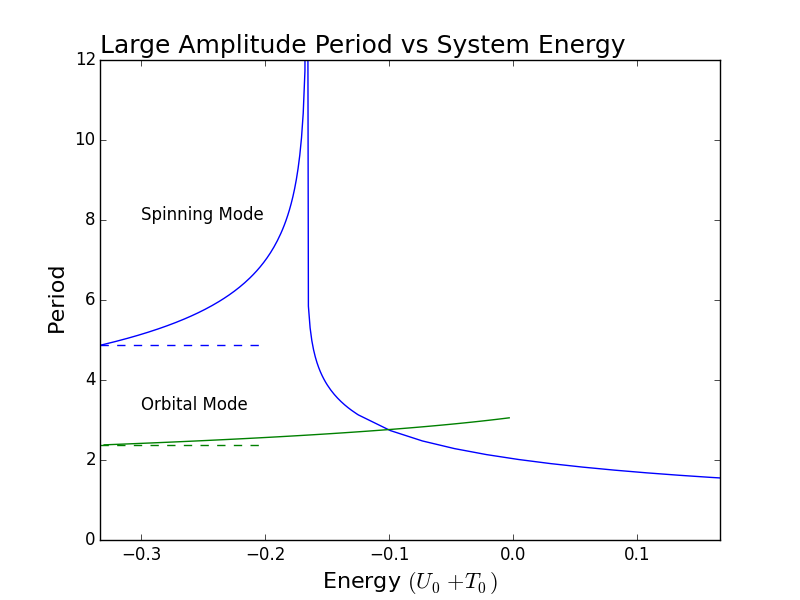
\includegraphics[width=0.85\textwidth]{./images/plot.png}
	\caption{Solid lines denote numerical results, dashed lines denote asymptotic small amplitude limit}
\end{figure}

\section{Conclusions}

In the analysis of this system so far we have found an interesting example of coupled non-linear hamiltonian that counter intuitively does not produce chaotic motion. However this is only the first of many questions this system leaves open for discussion. Using equation \ref{gen_ham} we can explore if this splitting of the hamiltonian works for any set of spheres or if there are certain proportionality's that must hold. We can also explore stability of circular orbits that likely exist. With the appropriate numerical techniques how these spheres interact with bouncing. These questions and more are available for examining.

\section{Acknowledgements}

I'd like to thank my peer Tyler Markham for expressing his opinions on the conveyance of various illustrations in this paper, my peer and Jacob Ciafre for listening to me speculate in our kitchen, Alice Haugen for prose editing and most importantly Amy Whillock for her patience and support.

%needed diagrams;
%numerical values of period vs energy
%geometry layout/labels
%animatique of basic modes
%revtek4.1

\bibliographystyle{plain}
\bibliography{./double_magnet_bib}


\end{document}
